% !TEX encoding = UTF-8 Unicode
% ------------------------------------------------------------------------------
% Este fichero es parte de la plantilla LaTeX para la realización de Proyectos
% Final de Grado, protegido bajo los términos de la licencia GFDL.
% Para más información, la licencia completa viene incluida en el
% fichero fdl-1.3.tex

% Copyright (C) 2012 SPI-FM. Universidad de Cádiz
% ------------------------------------------------------------------------------

En este capí­tulo tratarán los aspectos relacionados con la implementación del sistema, así como del entorno tecnológico usado para el desarrollo del mismo.

\section{Entorno de Construcción}\label{sec:entorno-construcción}

Como se ha especificado en la sección \ref{sec:arquitectura-fisica}, el desarrollo de este proyecto ha sido realizado haciendo uso del equipo del propio alumno, sin necesidad de alguna herramienta hardware extra. Para ello, se ha hecho uso de un marco tecnológico específico que se detallará a continuación: 

\paragraph*{Hardware}

Los elementos del hardware utilizados no son relevantes para el desarrollo del sistema, ya que no se requiere nada fuera de lo común en un equipo de trabajo convencional. En este caso, se ha utilizado un portátil MacBook Pro de 15 pulgadas, con procesador Intel Core i7 de 2.2 GHz y memoria RAM de 16GB 1333 MHz DDR3.

\paragraph*{IDE (Entorno de Desarrollo Integrado)}

NetBeans \cite{NetBeans} es un IDE libre y gratuito pensado especialmente en desarrollo de software bajo el uso del lenguaje de programación Java.

\paragraph*{Lenguaje de Programación} 

Para la realización de la aplicación web se ha utilizado el lenguaje de programación \textbf{Java}, en concreto la plataforma Java EE (Enterprise Edition), con la ayuda de varios frameworks para diferentes cometidos, como son JSF, PrimeFaces, EJB y JPA, que se describirán a continuación.

\paragraph*{Frameworks}

\begin{itemize}
\item \textbf{JSF (JavaServer Faces):} Framework MVC que proporciona un conjunto de componentes en forma de etiquetas definidas en páginas XHTML mediante el framework Facelets. Se utiliza para aplicaciones Java basadas en web simplificando el desarrollo de interfaces de usuario. 

\item \textbf{Facelets:} Framework basado que permite definir la estructura general de las páginas (su layout) mediante plantillas. Facelets se adapta perfectamente al enfoque de JSF y se incorpora a la especificación desde la revisión 2.1. La sustitución de JSP (JavaServer Pages) por Facelets como lenguaje básico para definir la disposición de las páginas permite separar perfectamente las responsabilidades de cada parte del framework. La estructura de la página se define utilizando las etiquetas Facelets y los componentes específicos que deben presentar los datos de la aplicación utilizando etiquetas JSF. Para más información sobre JSF y/o Facelets véase el enlace \cite{introduccionJSF} de la bibliografía.

\item \textbf{PrimeFaces:} Este framework es una extensión de JSF de código abierto que cuenta con un conjunto de componentes enriquecidos para facilitar la creación de interfaces de usuario \cite{PrimeFaces}.

\item \textbf{EJB (Enterprise JavaBeans):} Plataforma para construir aplicaciones empresariales portables, reusables y escalables, utilizando el lenguaje de programación java. EJB permite a los desarrolladores de aplicaciones enfocarse en construir la lógica de negocio sin la necesidad de gastar tiempo en la construcción de código de infraestructura \cite{EJB}. 

\item \textbf{JPA (Java Persistence API:} La persistencia dentro de EJB es administrada por JPA \cite{JPA}. Este framework permite persistir automáticamente los objetos Java utilizando una técnica denominada object-relational mapping (ORM). ORM es esencialmente el proceso de mapear la información contenida en los objetos Java hacia las tablas de base de datos utilizando una configuración.
JPA define un estándar para:

\begin{itemize}
\item La creación de configuración metadata del ORM para mapear entidades hacia tablas relacionales.
\item La EntityManager API, una API estándar para realizar las operaciones CRUD (create, read, update y delete) de las entidades.
\item El lenguaje Java Persistence Query Language (JPQL), para realizar búsquedas y obtener información persistida de la aplicación.
\end {itemize}

\end {itemize}

En la siguiente figura podemos ver una representación de la integración de los frameworks descritos en la arquitectura de 3 capas vista en la sección \ref{sec:arquitectura-logica}.

\vspace{10mm}

\begin{figure}[H]
\centering
  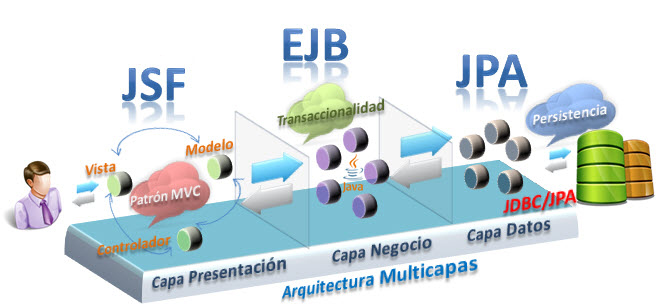
\includegraphics[scale=.60]{img/arquitectura-jee.jpg}
  \caption{\textit{Arquitectura de 3 Capas con Frameworks}}
  \label{fig:arquitectura-jee}
\end{figure}

\vspace{10mm}

\paragraph*{SGBD}

Se usará PostgreSQL, un sistema de gestión de bases de datos relacional orientado a objetos y libre. Como muchos otros proyectos de código abierto, el desarrollo de PostgreSQL no es manejado por una empresa o persona, sino que es dirigido por una comunidad de desarrolladores que trabajan de forma desinteresada, altruista, libre o apoyados por organizaciones comerciales \cite{PostgreSQL}.\\ 

Para administrar la base de datos PostgreSQL se ha utilizado la herramienta pgAdmin \cite{pgAdmin}.

\paragraph*{Control de Versiones}

De sobra es conocido que para la realización de grandes proyectos, o aquellos que sean de carácter importante, es casi obligatorio el uso de copias de seguridad. Comúnmente, se utiliza un sistema de control de versiones: cómodo, seguro y fácil de usar.\\

Para la realización de este proyecto se ha usado Git \cite{Git}, un sistema de control de versiones gratuito y de código abierto que garantiza confianza, eficacia y rapidez. Y en concreto, se ha usado la forja GitHub \cite{GitHub} para alojarlo.

\subsection{Entorno para la Web Pública}

No podemos olvidar que, aunque la documentación del proyecto se centre en la aplicación web del mismo, también se realiza un sitio web público para la empresa CoreSport \cite{CoreSport}.\\

Para la realización de esta web se ha utilizado el mismo equipo informático, pero distinto entorno software. En este caso, el IDE utilizado ha sido Brackets \cite{Brackets}, haciendo uso de HTML, CSS y JavaScript, como lenguajes para la realización de la web completa. Además, se ha usado el cliente FTP FileZilla \cite{FileZilla} para alojar la misma.


\section{Código Fuente}

El código del proyecto, llamado Booking, se ha estructurado principalmente en 2 módulos: uno de ellos, Booking-war, contendría todo lo relativo a la interfaz gráfica, incluyendo los controladores de páginas xhtml (JSF), y el otro, Booking-ejb, toda la parte EJB, incluyendo la persistencia JPA. La figura \ref{fig:estructura-ficheros} muestra la estructura general de los módulos y sus directorios principales. 

\begin{figure}
\centering
  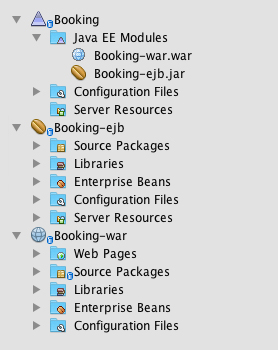
\includegraphics[scale=.65]{img/ficheros/estructura-ficheros.jpg}
  \caption{\textit{Estructura de los ficheros}}
  \label{fig:estructura-ficheros}
\end{figure}


\subsection{Módulo Web}

Veamos con algo más de detalle el módulo \textit{Booking-war}. Observamos que se compone de 5 directorios bien diferenciados:
\\

\textit{\textbf{Web Pages}}
\\

El primero de ellos hace referencia a los archivos de la interfaz de usuario, donde podemos distinguir por un lado el directorio \textit{WEB-INF}, por otro \textit{resources} y el resto de directorios que contienen todas las páginas XHTML divididas por carpetas dependientes del rol que el usuario posea. 

\begin{figure}
\centering
  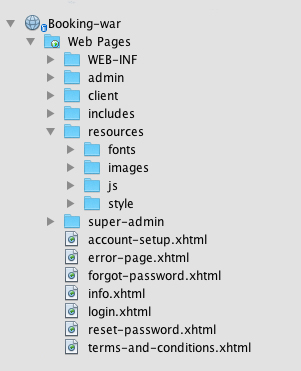
\includegraphics[scale=.60]{img/ficheros/web-pages.jpg}
  \caption{\textit{Directorio Web Pages}}
  \label{fig:ficheros-pages}
\end{figure}


\subparagraph{\textit{WEB-INF}}

Este directorio contiene, por una parte, todas las plantillas que se han creado para generar la interfaz de los distintos usuarios. Tendremos, por tanto, plantillas para los roles de superadministrador, administrador y usuario o cliente, además de las que estas usen por ser elementos en común, como pueden ser el footer (pie de página) o el selector de lenguaje. \\

Por otra parte, dentro de \textit{WEB-INF} cabe destacar dos ficheros: \textit{faces-config.xml} y \textit{web.xml}, accesibles también desde el directorio \textit{Configuration Files}. El primero de ellos se utiliza como fichero de configuración de idioma, donde se establece el idioma por defecto de la aplicación y aquellos que la misma soporta. En este caso se ha marcado el español como lenguaje por defecto, además de soportar el inglés, como vemos en su código: 

\lstinputlisting[language=XML]{ficheros/faces-config.xml} \label{file:faces-config}

\textit{web.xml} es un fichero de configuración donde podemos definir los parámetros principales de nuestra aplicación web, como pueden ser parámetros de autorización, redirecciones, tiempo máximo de sesión de usuario, gestión de errores, página de bienvenida por defecto, etc. \\

Así, podemos observar cómo se limita el acceso a los directorios dependiendo del rol del usuario: según la porción de código mostrada a continuación, ningún usuario estaría autorizado para acceder directamente a los archivos del directorio \textit{include}, y el superadministrador solo accedería a los de la carpeta con su nombre. Existe la misma regla para el resto de roles (administrador y usuario). Los archivos que permanecen en el directorio \textit{WEB-INF} sin incluirse en ningún subdirectorio sería accesible para todos los roles.

\lstinputlisting[language=XML, firstline=58, lastline=78]{ficheros/web.xml}

Vemos también a continuación un ejemplo de cómo se tratarían los errores, habiendo creado previamente una página XHTML pensada para tal fin (\textit{error-page.xhtml}):

\lstinputlisting[language=XML, firstline=120, lastline=134]{ficheros/web.xml}

O cómo se establece la página de expiración de sesión:

\lstinputlisting[language=XML, firstline=149, lastline=152]{ficheros/web.xml}

En esta última porción de código vemos que el archivo \textit{info.xhtml} acepta variables en la url, para indicar, en este caso, el tipo de información a mostrar. Así, el archivo nombrado mostrará información de sesión expirada, enlace expirado, o notificaciones del proceso para restablecer la contraseña olvidada. Este tipo de variables se usan en otras páginas de la aplicación, para consultar el perfil de algún usuario específico (siendo administrador para tener los permisos adecuados), ver los clases disponibles de un servicio o acciones de índole parecida donde se accede a los datos de una determinada instancia de una clase. 


\subparagraph{\textit{resources}}

Es el directorio que contiene todas las fuentes, imágenes, archivos JavaScript y hojas de estilo CSS de la aplicación. 


\subparagraph{\textit{admin, client, includes }y \textit{super-admin}}

Directorios que contienen todas las páginas xhtml de cada uno de los roles que su nombre indica, es decir, las páginas principales de la interfaz de usuario. La carpeta \textit{includes} contiene todas las páginas que son comunes a varios roles, accediendo a ella a través de algún archivo de su propia carpeta, como podemos ver en el siguiente ejemplo: 

\lstinputlisting[language=XML]{ficheros/services.xhtml}

Este archivo simplemente incluye la plantilla del cliente (menús y footer) y el archivo \textit{services-include.xhtml}, que contendrá el contenido del archivo para todos los roles.\\ 

Aquí podrían surgir dudas, ya que un superadministrador, un administrador y un cliente podrían tener distintas vistas en determinados ficheros, o simplemente tener más opciones disponibles en la vista de la tabla de clases de un determinado servicio, por ejemplo. Esto se gestionará dentro del archivo que se incluye limitando la vista de ciertos elementos a los roles que se autoricen: 

\lstinputlisting[language=XML, firstline=18, lastline=24]{ficheros/services-include.xhtml}

Siguiendo con el ejemplo de la vista de los servicios, el código anterior mostrará un botón para la creación de un nuevo servicio solo a los roles \textit{ADMIN} y \textit{SUPER\_ADMIN}, por lo que estará oculto cuando la vista sea destinada a un usuario del centro. \\

Además, puede llamar la atención el texto a mostrar en el botón: \textit{#\{txt['b\_new\_service']\}}. Como vimos anteriormente, en el fichero \textit{faces-config.xml} \ref{file:faces-config}, en el sistema se admiten dos idiomas, español e inglés. Pues bien, aquí está la clave para poder generar la interfaz en ambos idiomas -y los que se añadan en un futuro-. En la línea 14 del archivo mencionado se establece dónde encontrar los archivos de traducción: \textit{com.booking.language.text}. Mientras que la línea 15, muestra la variable a usar para realizar las traducciones: \textit{var}. Por lo que, cuando en los archivos XHTML encontramos código como el mostrado, el sistema tomará esa variable como una traducción e irá al directorio establecido en búsqueda del archivo del idioma seleccionado por el usuario, donde tomará el texto introducido para la variable en cuestión. En este caso, la variable sería \textit{b\_new\_service} y el texto equivalente para el idioma español \textit{Nuevo Servicio}, dado por la línea \textit{b\_new\_service=Nuevo Servicio} del fichero del lenguaje español de la ruta. Veremos estos archivos de idioma en unas líneas (\ref{lenguajes}).\\

Observamos en el código que el inicio de algunas etiquetas viene dado por una letra seguida de dos puntos. Esto indica qué tipo de elemento es el que le sigue a los dos puntos. Para ello, primeramente se incluye los paquetes necesarios: 

\lstinputlisting[language=XML, firstline=3, lastline=7]{ficheros/services-include.xhtml}

Por tanto, las opciones que se utilizan son: 

\begin{itemize}
\item h: elementos html convencionales.
\item ui: elementos del framework Facelets.
\item f: elementos propios de JSF.
\item p: elementos de PrimeFaces.
\end{itemize}
\\

\textbf{\textit{Source Packages}}
\\

\begin{figure}[H]
\centering
  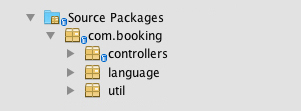
\includegraphics[scale=.70]{img/ficheros/source-packages.jpg}
  \caption{\textit{Directorio Source Packages}}
  \label{fig:source-packages}
\end{figure}


\subparagraph{\textit{controllers}}

Este directorio contiene los archivos Java principales asociados a la interfaz de usuario, los controladores. Cuando hablamos de JSF, el controlador Java asociado a cada página se denomina bean manejado o \textit{managed bean}, como su nomenclatura muestra en el código. Por tanto, cada uno de esos archivos XHTML usará, al menos, un controlador, el cual transmite los datos necesarios a la interfaz, actuando de puente con la gestión de la base de datos a través de EJB.

\lstinputlisting[language=Java, firstline=20, lastline=71]{ficheros/ServicesController.java}

Podemos observar que este bean Java es un bean manejado de JSF por su especificación en la línea 6 de código. Y, justo en la siguiente línea, se especifica el alcance del mismo (scope). Hay distintas opciones de scope para los beans: 

\begin{itemize}
\item ApplicationScoped: La información de este bean se guarda durante toda la vida de la aplicación web, desde que se ejecuta por primera vez hasta que se elimina del servidor. 
\item SessionScoped: Se puede intuir por el nombre que son beans de sesión, es decir, la información se mantiene desde que un usuario comienza una sesión en la aplicación hasta que esta acaba.
\item ViewScoped: La información perdura el tiempo de vista de una página, o sea, desde que el usuario accede a la misma hasta que se navega a una distinta. Disponible desde JSF 2.0.
\item RequestScoped: La vida del bean empieza cuando se produce una petición al servidor y acaba cuando el usuario recibe la respuesta con la información pedida. Por tanto, se creará una instancia del bean en cada petición al servidor.
\item NoneScoped: Este bean se instancia cuando es invocado por otro bean, siendo eliminado cuando la necesidad acabe.
\item CustomScoped: Desde JSF 2.0 también es posible la creación de scopes personalizados, donde se podrá configurar el tiempo del mismo. 
\end{itemize}

Vemos también el uso de clases EJB en las líneas 10-17, clases que se encargarán de la consulta o edición de la información de nuestra base de datos. Por tanto, los controladores harán uso de las funciones de estas clases cada vez que se requiera hacer uso de la BD, como en la línea 36, donde se realiza una consulta de todos los servicios de la empresa, o en la 40, que se invoca a la función encargada de activar un servicio que estaba suspendido. 


\subparagraph{\textit{language}} \label{lenguajes}

Como su nombre indica, este directorio contendrá los archivos de los distintos lenguajes que el sistema soporta. Existirá un archivo de extension \textit{.properties} por cada lenguaje. Como se vio en \ref{file:faces-config}, se establece un nombre de archivo base para los ficheros de texto:

\lstinputlisting[language=XML, firstline=14, lastline=14]{ficheros/faces-config.xml}

Así, existirá un archivo con el nombre base \textit{text.properties} que el sistema consultará en caso de no encontrar la traducción en el archivo de idioma específico o algún otro error similar. En esta aplicación, por tanto, tendremos tres archivos en la carpeta: \textit{text.properties}, \textit{text\_en.properties} y \textit{text\_es.properties}, donde los dos últimos serían los archivos de traducción para inglés y español, donde observamos que toman el nombre base especificado añadiendo el código del idioma que representan. En la figura \ref{fig:comparacion-lenguajes} vemos un ejemplo de traducción para las mismas palabras, a las cuales se accederán en las vistas XHTML mediante la variable \textit{var} como vimos anteriormente.

\begin{figure}
\centering
  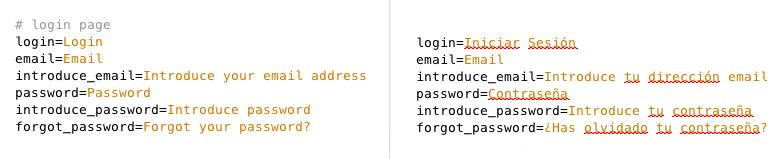
\includegraphics[scale=.60]{img/comparacion-lenguajes.jpg}
  \caption{\textit{Directorio Comparativa de Lenguajes}}
  \label{fig:comparacion-lenguajes}
\end{figure}


\subparagraph{\textit{util}}

El directorio \texit{util} se utiliza para almacenar todas aquellas clases que se han creado pensadas en ser una ayuda en cualquier parte de la aplicación, como por ejemplo, \texit{DateService}, mediante la cual se realizan gestiones de fechas (como devolver una fecha con hora 00:01, usada para búsquedas), \texit{Constant}, que incluye algunas variables constantes usadas en toda la aplicación, o \texit{FacesUtil}, que es la clase más usada de este directorio, mediante la cual podemos acceder a diversas funciones, como obtener o establecer atributos de sesión, obtener la dirección IP en uso, añadir mensajes en la vista actual, saber quién es el usuario haciendo uso de la aplicación o realizar redirecciones.\\
\\

\textbf{\textit{Libraries, Enterprise Beans} y \textit{Configuration Files}}
\\

\begin{figure}
\centering
  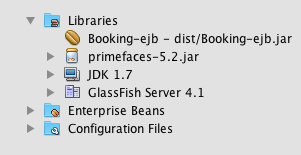
\includegraphics[scale=.70]{img/ficheros/otros-directorios-web.jpg}
  \caption{\textit{Directorios Libraries, Enterprise Beans y Configuration Files}}
  \label{fig:otros-directorios-web}
\end{figure}

\subparagraph{\textit{Libraries}}

Como su nombre indica, contiene todas las librerías/dependencias que este módulo usa, incluyendo el módulo \textit{Booking-ejb}. JDK (Java), PrimeFaces y GlassFish completarían la lista. \\

\subparagraph{\textit{Enterprise Beans}} 

Es simplemente una carpeta que contiene todas las clases EJB que utiliza el módulo \textit{Booking-war}, es decir, todas las \textit{Facades} de las que hace uso para acceso a la información de la BD. \\

\subparagraph{\textit{Configuration Files}} 

Posee los archivos de configuración de este módulo, como los ya vistos \textit{faces-config.xml} y \textit{web.xml} u otros destinados al servidor (\textit{glassfish-web.xml}).


\subsection{Módulo EJB}

\begin{figure}
\centering
  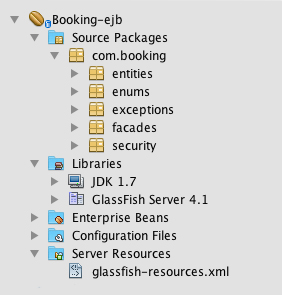
\includegraphics[scale=.70]{img/ficheros/ficheros-ejb.jpg}
  \caption{\textit{Directorios módulo Booking-ejb}}
  \label{fig:ficheros-ejb}
\end{figure}

Este módulo se centra en la gestión de las clases necesarias para la solución buscada para el proyecto, las cuales hemos visto en el diagrama conceptual de clases UML \ref{fig:modelo-conceptual}, así como su mapeo respecto a las clases creadas en la base de datos y la gestión de todo ello. La estructura del mismo es similar a la del módulo que acabamos de ver: 
\\

\textbf{\textit{Source Packages}}
\\

Este sería el directorio principal del módulo, donde se establecen los paquetes del mismo. Así, tendremos los siguientes paquetes que vamos a ir describiendo: 

\begin{itemize}
\item \textbf{\textit{entities}}: El cual contiene todas las clases utilizadas en el sistema, incluyendo las que surgen de las relaciones entre las clases del modelo conceptual UML, como puede ser el case de \textit{Booking}, una clase que aparece de la relación entre las clases \textit{ActivityClass} (Clase) y \textit{User} (Usuario), conteniendo la instancia de ambos cada vez que se realiza una reserva de la clase de un servicio (entrenamiento funcional, TRX, pilates, etc.). Veremos un ejemplo de entidad en la sección \ref{subsec:entities}.
\item \textbf{\textit{enums}}: Directorio con las clases \textit{enum} del sistema, como los estados, tipos de notificaciones o roles.
\item \textbf{\textit{exceptions}}: Conjunto de excepciones creadas para el manejo del programa.
\item \textbf{\textit{facades}}: Este directorio, junto con \textit{entities}, toma el protagonismo de los paquetes del módulo. Contiene todas las clases que realizan la gestión de los datos, tanto funciones CRUD (Crear, Leer, Actualizar y Borrar) como consultas. Por tanto, a cada una de las entidades creadas le corresponderá una clase \textit{Facade} para su gestión en la base de datos, como veremos a continuación en la sección \ref{subsec:facades}.
\item \textbf{\textit{security}}: Contiene el archivo de codificación de contraseñas con el algoritmo a usar en el momento de almacenar la misma en la BD y las funciones para las verificaciones oportunas en el inicio de sesión de los usuarios.
\end{itemize}
\\

\textbf{\textit{Libraries, Enterprise Beans, Configuration Files} y \textit{Server Resources}}
\\

El resto de directorios que componen el módulo EJB son los siguientes:

\subparagraph{\textit{Libraries}}

Librerías/dependencias que este módulo usa. En este caso, JDK (Java) y GlassFish. \\

\subparagraph{\textit{Enterprise Beans}} 

Es simplemente una carpeta que contiene todas las \textit{Facades} EJB generadas. \\

\subparagraph{\textit{Configuration Files}} 

Posee archivos de configuración de este módulo, como por ejemplo \textit{persistence.xml}, archivo de persistencia JDBC (framework usado por JPA).

\subparagraph{\textit{Server Resources}} 

Podemos destacar el único fichero que posee este directorio, \textit{glassfish-resources.xml}, a través del cual este módulo, y por tanto la aplicación, configura la conexión con el servidor GlassFish, indicando el puerto de conexión, la base de datos utilizada, datos de acceso, etc., como vemos en su código.

\lstinputlisting[language=XML]{ficheros/glassfish-resources.xml}


\section{Gestión de Base de Datos} \label{sec:gestion-bd}

\textit{Java Persistence API} (JPA) es el acceso estándar a bases de datos relacionales en Java EE. Provee una forma simple y eficiente de gestionar el ORM (\textit{object/relational mapping}) de objetos Java (\textit{POJO}) respecto a los datos de la BD. Hablamos de las entidades JPA, o nuestras \textit{entities} que acabamos de describir. \\

Cada entidad se asocia (aunque no en el 100\% de los casos) a una tabla relacional de la BD, por lo que cada instancia de una entidad quedará representada por una fila de esa tabla. Estas entidades establecen diferentes relaciones entre ellas: \textit{one-to-one, one-to-many, many-to-one} o \textit{many-to-many}. Por tanto, las aplicaciones Java que gestionan estas entidades se ven en la necesidad de acceder y navegar por las instancias y sus relaciones. Y esta necesidad se satisface con JPQL (\textit{Java Persistenece Query Language}).\\

Vayamos por partes; centrándonos en nuestro código, hemos comprobado que el módulo EJB contiene los ficheros responsables de la gestión de base de datos. De acuerdo a lo afirmado en los párrafos iniciales de esta sección, podemos centrarnos en los paquetes \textit{com.booking.entities} y \textit{com.booking.facades} del mismo. \\

\subsection{\textit{Entities}} \label{subsec:entities}

Empecemos con el ejemplo de la clase de java \textit{Service}.

\lstinputlisting[language=XML, firstline=25, lastline=48]{ficheros/Service.java}

Observamos cómo se establece la correspondencia de las entidades Java con las clases de la base de datos (ORM). De esta manera, la elección y uso del SGBD será independiente a nuestro código, simplemente habría que crear las clases y atributos con los nombres que definimos en las entidades. Así, para la clase \textit{Service} tendremos una tabla \textit{services} en la BD, con los atributos \textit{id, name, description, organisation, status} y \textit{created\_date}, correspondientes a los atributos \textit{id, name, description, organisation, status} y \textit{createdDate} de nuestra clase Java \textit{Service}. \\

Puede llamar la atención la estrategia de generación del atributo \textit{id}: \textit{@GeneratedValue(strategy = GenerationType.IDENTITY)}. Estos se crearán automáticamente en la BD, siguiendo un orden estándar, desde el número 1, por lo que no tendremos que gestionar los identificadores de las instancias de las clases. \\

Además, hemos observado que aparece una organización en el sistema. Puede parecer algo redundante al tratarse de una aplicación web para un centro de entrenamiento y empresa específicos. Aun siendo esto cierto, la programación del sistema se ha realizado pensando en la escalabilidad y teniendo en cuenta la posibilidad de que, en un futuro, otro centro similar puede hacer uso de la misma, incluso compartiendo el mismo servidor y la misma base de datos. De ahí que se gestione toda la información haciendo distinción de la organización a la que pertenece, así se podrán añadir otras empresas con pequeños adaptaciones en el sistema, teniendo cada una de ellas sus propias características, personalizando el logo o el estilo de la interfaz de usuario.

\subsection{\textit{Facades}}\label{subsec:facades}

Como se ha afirmado antes, a cada entidad le corresponderá un archivo \textit{Facade} para las funciones pertinentes. 

\lstinputlisting[language=XML, firstline=17, lastline=47]{ficheros/ServiceFacade.java}

Así, la 'fachada' \textit{ServiceFacade} contiene los métodos \textit{createNewService, updateService, activateService} y \textit{deactivateService} que los controladores (beans manejados) usarán para el acceso a la BD. \\

Aparte de estas funciones CRUD, también será la clase encargada de realizar las consultas SQL de cada entidad a través de JPQL, como vemos en los siguientes ejemplos: 

\lstinputlisting[language=XML, firstline=77, lastline=81]{ficheros/ServiceFacade.java}

\lstinputlisting[language=XML, firstline=89, lastline=93]{ficheros/ServiceFacade.java}

Gracias al uso de JPQL y al mapeo realizado, en la nomenclatura de las consultas se usa las clases y atributos Java, y no el nombre correspondiente de la base de datos. Este método de consulta facilita tanto la realización de las mismas por parte del programador como, de nuevo, la independencia del SGBD elegido o los cambios que puedan hacerse en el mismo. 


\subsection{Sistema de Gestión de Base de Datos (SGBD)}

Como ya se ha informado, el SGBD elegido para llevar a cabo este proyecto ha sido \textit{PostgreSQL}. \textit{PostgreSQL}, o simplemente Postgres, es un sistema de gestión de bases da datos relacional orientado a objetos dirigido por una comunidad de desarrolladores que la gestionan de forma libre y altruista o mediante organizaciones comerciales. Está considerado el SGBD de código abierto más potente del mercado. \textit{pgAdmin} es la herramienta oficial para administrar las bases de datos en PostgreSQL, y la que se ha usado en este caso. \\

Las característcas y ventajas del uso de PostgreSQL son las siguientes: 

\begin{itemize}
\item Ahorros considerables de costos de operación: Diseñado con las características, estabilidad y rendimiento de grandes proveedores comerciales con un menor mantenimiento.
\item Estabilidad y confiabilidad. 
\item Extensible: Debido a la disponibilidad de su código fuente aquel que lo requiera podría extender o personalizar el programa de acuerdo a sus necesidades.
\item Multiplataforma, incluyendo Linux, Windows, Unix, Solaris y MacOS X.
\item Estrategia de almacenamiento MVCC (Control de Concurrencias Multiversión): Consigue una mejor respuesta en grandes volúmenes de información, además de permitir acceso de solo lectura durante la edición de registros, dando la opción de realizar copias de seguridad en caliente.
\item Herramientas gráficas de diseño y administración de bases de datos.
\item Soporta tanto los tipos de datos, cláusulas, funciones y comandos estándar SQL92/SQL99 como los extendidos por el propio PostgreSQL.
\item Buen sistema de seguridad.
\item Gran capacidad de almacenamiento.
\item Buena escalabilidad, soportando mayor cantidad de peticiones simultáneas a BD ajustándose a la CPU y cantidad de memoria disponible de forma óptima.
\item Soporta claves ajenas (\tesxtit{foreign keys}), disparadores (\tesxtit{triggers}), vistas, integridad transacional, herencia de tablas, tipos de datos y operaciones geométricas, transacciones distribuidas, afirmaciones(\tesxtit{assertions}), etc.
\end{itemize}

Volviendo a nuestro sistema, un ejemplo de script de creación de una tabla de la BD sería: 

\begin{lstlisting}[language=SQL, showspaces=false]
CREATE TABLE schema_booking.services
(
  id serial NOT NULL,
  created_date timestamp without time zone,
  description character varying(255),
  name character varying(255),
  status character varying(255),
  organisation bigint,
  CONSTRAINT services_pkey PRIMARY KEY (id),
  CONSTRAINT fk_services_organisation FOREIGN KEY (organisation)
      REFERENCES schema_booking.organisations (id) MATCH SIMPLE
      ON UPDATE NO ACTION ON DELETE NO ACTION
)
WITH (
  OIDS=FALSE
);
ALTER TABLE schema_booking.services
  OWNER TO booking;
\end{lstlisting}

Y la representación de dos instancias de la entidad \tesxtit{Service} en la tabla \tesxtit{services}:

\begin{figure}[H]
\centering
  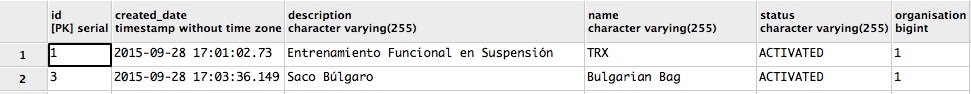
\includegraphics[scale=.50]{img/services-rows.jpg}
  \caption{\textit{Instancias de Service en la tabla Services}}
  \label{fig:services-rows}
\end{figure}












